\documentclass{endm}
\usepackage{endmmacro}
\usepackage{graphicx}


\usepackage{amssymb,amsmath,latexsym}
\usepackage[varg]{pxfonts}
%%%%%% ENTER ADDITIONAL PACKAGES
%\usepackage{graphics}
\usepackage{pst-all}
\usepackage{graphicx}
\usepackage{amsmath,amsfonts}
\usepackage{amssymb} % ADDED
\usepackage{times}
\usepackage{latexsym}
\usepackage{fancybox}
\usepackage{algorithm}
%\usepackage{algorithmic}
\usepackage{algorithmicx}
\usepackage{algpseudocode}
\usepackage{setspace}
\usepackage{courier}
\usepackage{verbatim}
\usepackage{hhline}
\usepackage{etex}
\usepackage{tikz}
\usetikzlibrary{calc,arrows,automata}
\usetikzlibrary{matrix,positioning,arrows,decorations.pathmorphing,shapes}
\usetikzlibrary{shapes,snakes}
%---------------hola
\usepackage{subfigure}
\usepackage{mathtools}
\usepackage{booktabs}
\usepackage{hyperref}

\tolerance=1
\emergencystretch=\maxdimen
\hyphenpenalty=10000
\hbadness=10000


\floatname{algorithm}{Algorithm}


\def\lastname{Please list your Lastname here}

\begin{document}

% DO NOT REMOVE: Creates space for Elsevier logo, ScienceDirect logo
% and ENDM logo
\begin{verbatim}\end{verbatim}\vspace{2.5cm}

\begin{frontmatter}

\title{An Approximation Algorithm for the Two-Node-Connected Star Problem with Steiner Nodes}

\author{Graciela Ferreira Leites Mundell (1551496-1),}
\author{Franco Rafael Robledo Amoza (3645500-3),}
\author{Pablo Gabriel Romero Rodr\'iguez (3702465-5)}

\address{Instituto de Matem\'atica y Estad\'istica\\ Facultad de Ingenier\'ia. Universidad de la Rep\'ublica\\ Montevideo, Uruguay}
\thanks[mails]{Emails:\href{mailto:gferreira@fing.edu.uy} {\texttt{\normalshape
   \{gferreira,frobledo,promero\}@fing.edu.uy}}}

\begin{abstract}
\setlength{\parindent}{12pt}
The goal in topological network design is to build a minimum-cost topology meeting specific real-life constraints.
There is a cost-robustness trade-off under single and multiple failures.

Previous works in the field suggest that a backbone composed by a two-node-connected toplogy provides savings with respect to elementary cycles.
Consequently, we introduce the Two-Node Connected Star Problem with Steiner Nodes (2NCSP-SN). The goal is to design a minimum-cost topology,
where the backbone is two-node connected, the access network is connected in a \emph{star} topology or by direct links to the backbone,
and optional nodes (called Steiner nodes) could be included in the solution. The 2NCSP-SN belongs to the class of $\mathcal{NP}$-Hard problems.
This promotes the development of heuristics and approximation algorithms.

An approximation algorithm of factor $4\alpha$ for the 2NCSP-SN is introduced, being $\alpha \geq 1/2$ the cost-ratio between backbone and access links.
This is a generalization of the well-known factor 2 for the design of minimum-cost two-connected spanning networks (if we fix $\alpha=1/2$).
Finally, an exact Integer Linear Programming (ILP) formulation is proposed in order to highlight the effectiveness of the approximation algorithm.
The results confirm a small gap between the globally optimum solution and the topology offered by our approximation algorithm when the ratio $\alpha$ is close to $1/2$.
\end{abstract}

\begin{keyword}
Network Optimization, Approximation Algorithm, Integer Linear Programming
\end{keyword}

\end{frontmatter}

\begin{figure}
  \caption{A picture of a gull.}
  \centering
    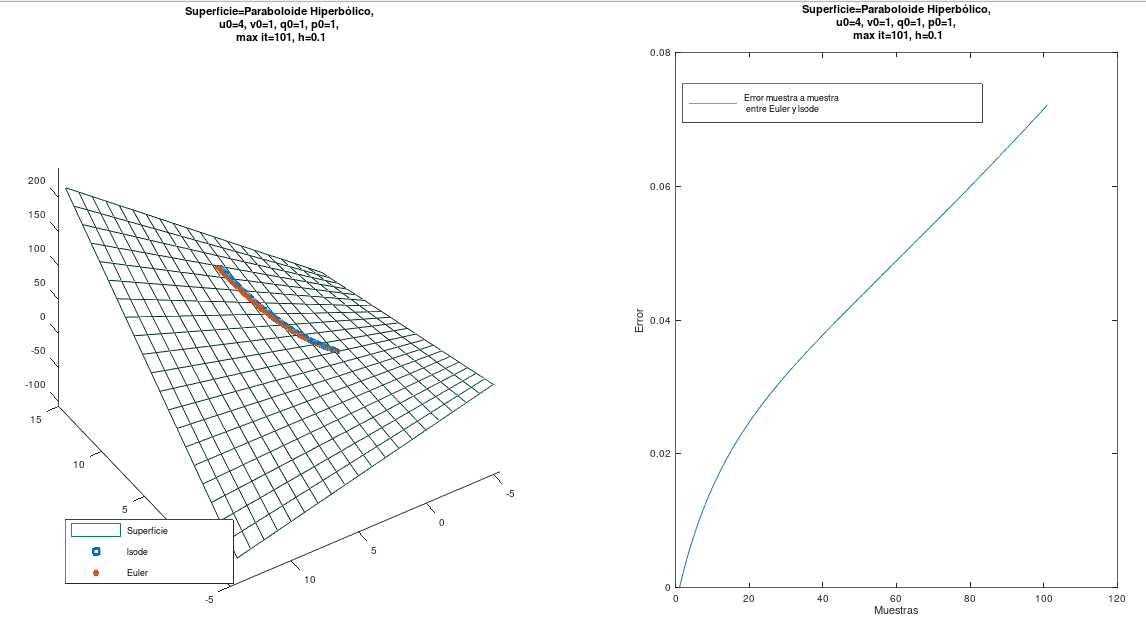
\includegraphics[width=\textwidth]{ph.eps}
\end{figure}
\section{Introduction}\label{intro}
The minimum-cost toplogy meeting simple connectivity is the Minimum Spanning Tree, or MST. In this basic setting, Greedy algorithm efficiently finds the MST~\cite{Kruskal}.
However, the design of communication systems is more challenging, since the cost-redundancy trade-off should be tackled.
In the physical layer, this means that the network must be robust under single failures of any component, or two-node connected.

A natural way to connect terminal nodes in order to fulfill two-connectivity is to consider an elementary cycle. The design of a minimum-cost
elementary cycle is a celebrated problem, known as the Travelling Salesman Problem or TSP. Supported by the concept of reducitibility
and Karp list, it is well-known that the TSP belongs to the class of $\mathcal{NP}$-Hard problems~\cite{Karp72}.
Indeed, a natural reduction to Hamiltonian tour is obtained using $0$-$1$ costs in their links.

A foundational work credited by Clyde Monma et. al. confirms that elementary cycles are sub-optimal for the design of
minimum-weight 2-node-connected spanning network problem or MW2CSNP~\cite{monma1990minimum}.
However, the authors show that cost of the cheapest Hamiltonian tour, $C_{\mathcal{H}}$, always respects the inequality
$C_{\mathcal{H}} \leq 4/3 OPT$, being $OPT$ the cost of the globally optimum solution.
Furthermore, the bound is tight, since they build an asymptotic family of graphs such that the cost-ratio tends to $4/3$. The authors find structural properties of the globally optimum
solution for the MW2CSNP and, they remark that the optimum 2-edge connected is also
2-node connected. The MW2CSNP is at least as hard as the TSP (using $0$-$1$ costs, $OPT$ is not greater than the number of nodes
iff the graph is Hamiltonian). Therefore, several authors address the MW2CSNP using heuristics and approximation algorithms.
Christofides provides a $3/2$-factor for metric TSP which, together with the $4/3$ factor credited by
Monma et. al. results in an approximation algorithm with factor $2$ for the MW2CSNP~\cite{christofides}. This factor-$2$ can be extended to
several topological network design problems such as Steiner Networks, using either combinatorial analysis or strong duality
theorem from linear programming~\cite{vazirani2003approximation,GW}.

The physical implementation of fiber-optics communication imposed a new challenge, \emph{geographical diversity}. As a consequence,
real-life communication networks are hierarchically structured in a backbone and access network, where customers in the last-mile
have elementary connectivity requirements~\cite{robledo2005grasp}. Martine Labb\'e et. al. introduced
a hierarquically organized network, called Ring Star Problem, where the backbone is a ring and the access network is a \emph{star},
this is, direct links connected to the ring~\cite{labbe2004ring}. A natural topological extension called Two-Node Connected Star Problem (2NCSP)
has been introduced by Recoba et. al.~\cite{recoba2016two}.
The ring is replaced by an arbitrary two-node connected topology, and
the authors confirm savings with respect to optimal solutions for the RSP (which are in turn feasible for the 2NCSP). Here, an extension of the 2NCSP is proposed, by the introduction of optional Steiner nodes in feasible solutions. 

\textbf{\emph{Complexity}}: Being RSP and 2NCSP $\mathcal{NP}$-Hard problems, 2NCSP-SN is $\mathcal{NP}$-Hard too.


The contributions of this article are the following:
\begin{itemize}
\item The Two-Node-Connected Star Problem with Steiner Nodes (2NCSP-SN) is here introduced.
\item A generalization of the factor-2 result is offered. Specifically, an approximation algorithm with factor $4\alpha$ is
introduced for the 2NCSP, being $\alpha \geq 1/2$ the relation between the link-costs from the backbone/access network.
\item An exact Integer Linear Programming (ILP) formulation for the 2NCSP-SN is presented.
\item A sensibility analysis is carried out in order to understand the effectiveness of
our approximation algorithm.
%The reason is to determine whether the algorithm returns near-optimal or feasible solutions close to the factor $4 \beta$.
\end{itemize}

The paper is organized as follows. Section~\ref{Problem} formally presents the 2NCSP-SN using an ILP formulation.
An approximation algorithm with factor $4\alpha$ is introduced in Section~\ref{AA}.
A fair comparison between the globally optimum solution and the approximation algorithm is performed in Section~\ref{Comparison}.
Finally, Section~\ref{Conclusions} presents concluding remarks and trends for future work.

\section{Problem}\label{Problem}
We are given a simple graph $G = (V,E)$, internal link-costs $IC = \{c_{e}\}_{e\in E}$, external link-costs $EC = \{d_{e}\}_{e\in E}$, and $V=S\cup T$, being $T$ the terminal-set and
$S$ Steiner nodes with costs $\{a(s)\}_{s\in S}$. The goal in 2NCSP-SN is to build a minimum-cost spanning subgraph $H = (V_H,E_H)$, where $T \subseteq V_H$ and $V_H = I \cup L$, being $L$ the set of leaf-nodes (in the access network), such that $deg_{H}(v) = 1, \forall v\in L$, and
the induced subgraph $H(I)$ is two-node-connected.

%The objective function
%is the constribution of internal/external connections and Steiner nodes:
%$c(H)=\sum_{e\in E_H(I)}c(e)+\sum_{e\in E_H(L)}d(e)+\sum_{s\in S\cap V_H}c(s)$.

%Let $Q=\{q=(i,j),\forall i,j \in T\}$ be the set of all pairs of nodes in $T \subseteq V$. For each $q \in Q$ we define $G^{q}=(V^{q},E)$, where $V^{q}=T(q)\cup S(q)$ with $T(q)=\{o(q),d(q)\}$  and $S(q)=S\cup (T \setminus T(q))$.  In order to model survivability conditions on the network core, we introduce a minimal cost flow problem,over each network $G^{q}$ with capacity constraints. If both terminal nodes $q$ are in the backbone then  two node connectivity are required between them, in other case only a simple path is required.% additional integer variables are need. As we introduce a flow conditions we need work with directed graphs. Let $Gd^{q}=(V^{q},Ed)$ be the directed graph built from $G^{q}=(V^{q},E)$.%,such that for each link $e=(i,j)\in E, \forall e\in E, \forall i,j \in V^{q}$ two arcs are added in $Gd^{q}$ one from node $i$ to node $j$ and other from $j$ to $i$.

Let us develop an ILP for the problem under study. The key idea is to consider connectivity requirement $r_q=2$ for every pair of terminals $q$ from the backbone, while $r_q=1$ otherwise.
Let $Q=\{q=(i,j),\forall i\neq j, i,j \in T\subseteq V\}$. Consider the following set of binary variables:
\begin{itemize}
\item  $z_{ij}=1$ iff $(i,j)\in E$ is in the backbone;
\item $y_{ij}=1$ iff $(i,j)\in E$ is in the access network;
\item $x_{ij}^{q}$ is the $i-j$ flow for every pair of terminals $q$;
\item $p_{i}=1$ iff the $i$ is included in the access network.
\end{itemize}

An ILP formulation for the 2NCSP-SN can be expressed as follows:

%TODO PASAR A FORMATO ALIGN; ACOMODAR EN UNA SOLA RESTRICCION LA QUE APARECE CON LLAVES
\setcounter{equation}{0}
\begin{align}
\small
\mbox{min}_{H \subseteq G} &c(H)= \sum _{ij\in E} c_{ij}.z_{ij}+ \sum _{s\in S} a_{s}.p_{s}+ \sum _{ij\in E} d_{ij}.y_{ij}\label{ecu0} \\
\mbox{s.t.} &\sum _{j:(j,i)\in E} x_{ji}^{q}-\sum _{j:(i,j)\in Ed^{q}} x_{ij}^{q} =  I(i).r_{i}\: \forall i \in V,\:\forall q=(q_{o},q_{d})\in Q \label{ecu1}\\
& I(i)=1 \:\forall i \in V \backslash \{q_{o}\},\:I(q_{o})=-1 \label{ecu2}\\
& r_{i}= 0 \:\forall i \in V \backslash \{q_{o},q_{d}\} \label{ecu3}\\
& \max(1,p_{q_{o}}+p_{q_{d}}) \leq r_{i}\leq 1+ \min(p_{q_{o}},p_{q_{d}}),\:\forall  i \in \{q_{o},q_{d}\},\:\forall q\in Q\label{ecu4}\\
& x_{ij}^{q}+x_{ji}^{q} \leq z_{ij}+y_{ij},  \:\forall ij\in E,\:\forall q \in Q \label{ecu5}\\
& \sum_{j \in \delta (i)} y_{ij} \leq  1+ M p_{i}, \:\forall  i\in T \label{ecu6}\\
&\sum _{j\in \delta (i)} (z_{ij}+y_{ij}) \leq  M p_{i}, \:\forall  i\in S \label{ecu7}\\
& y_{ij} \leq 2-p_{i}-p_{j}, \: \forall ij\in E, i,j \in V\label{ecu8}\\
& z_{ij} \leq \min(p_{i},p_{j}), \: \forall ij\in E, i,j \in V\label{ecu9}\\
& z_{ij}+y_{ij} \leq 1 \: \forall ij\in E, i,j \label{ecu10}\\
& 2p_{i} \leq \sum_{j\in \delta (i)}z_{ij}\leq Mp_{i}, \: \forall i \in V\label{ecu11}
\end{align}

Where $\delta (i)$ is neighbor-set for node $i$, and $M$ is an arbitrarily large integer.
The objective function~\eqref{ecu0} is the contribution of internal/external connections and Steiner nodes. Constraints~\eqref{ecu1}-\eqref{ecu4} ensure connectivity using Kirchhoff equations.
%When the pair of terminals $q$ belongs to the backbone, $r_{i}=2, i\in \{q_{o},q_{d}\}$;
%otherwise $r_{i}=1$.
Constraints~\eqref{ecu5}~and~\eqref{ecu6} force one-way flow.
By Constraint~\eqref{ecu7}, optional Steiner nodes belong to the backbone, if needed.
The definitions of binary variables $y_{ij}$ and $z_{ij}$ are captured by Constraints~\eqref{ecu8}
and~\eqref{ecu9}. Constraints~\eqref{ecu10} state that either $y_{ij}$  or $z_{ij}$ can be set to $1$, but not both. 
Constraints~\eqref{ecu11} state that a terminal from the backbone could have multilinks, but nodes from the access network have one link.

\section{Methodology}\label{AA}
From now on, we assume that the internal/external costs are positive and internal costs satisfy the triangle inequality. Without loss of generality, a complete graph $G=(V,E)$ is considered. Let $\alpha_{e}=\frac{c_e}{d_e}, \forall e \in E$ be the primary/secondary cost ratio for each arc.
In this section we build an approximation algorithm for the the 2NCSP-SN of factor $4\alpha$,
being $\alpha$:
\begin{equation}
\alpha = \max_{e\in E} \left\{\alpha_{e} \right\}
\end{equation}

Recall that Christofides's algorithm is a 3/2-factor for the metric TSP.
The key concept of our approximation algorithm is Christofides in order to span the terminal-set
with an elementary cycle. Greedy augmentations of the solution including Steiner nodes also takes place, whenever the cost is reduced.

In Line~1, $Christofides$ is called in order to build an elementary cycle $\mathcal{C}$
that spans the terminal-set $T$. The corresponding solution is updated in Lines 2-3,
where the backbone is $\mathcal{C}$ and the access network is empty yet.
In the while-loop (Lines 4-11),
Steiner nodes are greedily included in the backbone, whenever the cost is reduced (Line 5).
If this happens, some terminal node $v$ is included in the access network, and the
evidence $s \in S$ is added to the backbone (Lines 6-7). Observe that candidate terminals
$t \in T$ are iteratively checked (Line 9), and the condition $|J|\geq 3$ forces to have
a cycle in the backbone. The corresponding feasible solution $F$ is finally returned (Line 12).

\begin{algorithm}[H]
\small
\centering
\begin{algorithmic}[1]
\Require $G=(T\cup S,E)$,$c(e),d(e) \forall e \in E$,
\State {$\mathcal{C} \leftarrow Christofides(G,c)$ }
\State {$L \leftarrow \emptyset$, $I \leftarrow T$, $E^{\prime} \leftarrow E(\mathcal{C})$, $J \leftarrow T$}
\State {$F \leftarrow (L\cup I,E^{\prime})$}
%\Comment {Introduce Steiner nodes to the Backbone if the cost is reduced:}
\While{$|J| \geq 3$}
    \If {there are  $s \in S$, $(t,v),(v,w)\in F$: $c(t,v)+c(v,w)>d(v,s)+c(t,s)+c(s,w)$}
            \State {$L \leftarrow L\cup \{v\}$, $I \leftarrow I \cup \{s\}\:  \backslash\: \{v\}$, $J \leftarrow J \backslash \{t,v\}$ }
            \State {$E^{\prime} \leftarrow E^{\prime} \cup \{(t,s),(s,v),(s,w)\}\:\backslash\: \{(t,v),(v,w)\} $ }
         \Else
           \State {$J \leftarrow J \:\backslash\: \{t\}$}
    \EndIf
\EndWhile \\
\Return $F=(I\cup L,E^{\prime})$
\end{algorithmic}
\end{algorithm}

\clearpage

\begin{lem}\label{lema}
If $L(F) \neq \emptyset$ then $\alpha>1/2$
\end{lem}
\begin{proof}
By the triangle inequality, $c_{(t,v)}\leq c_{(t,s)}+c_{(s,v)}$ and
$c_{(v,w)}\leq c_{(v,s)}+c_{(s,w)}$, so
$c_{(t,v)}+c_{(v,w)} \leq c_{(t,s)}+2.c_{(s,v)}+ c_{(s,w)}$. If $L \neq \emptyset$, there exists $v \in L$, $s \in S \cap I, t,w \in I$ such that
$c_{(t,v)}+c_{(v,w)}>d_{(v,s)}+c_{(t,s)}+c_{(s,w)}$,\\ %\, d_{(v,s)}= c_{(v,s)}/\alpha$.\\
Therefore $d_{(v,s)} = c_{(v,s)}/\alpha_{v,s }< 2.c_{(s,v)}$, so there exists $e=(v,s)$ such that $\alpha_{e} > 1/2$, that is $\alpha > 1/2$ with $\alpha = \max_{e\in E} \left\{\alpha_{e} \right\}$.

\end{proof}
%According to Lemma~\ref{lema}, if $\alpha \geq 2$ then $F$ is an elementary cycle without Steiner nodes.
\begin{thm}
$c(F) \leq \max\{2,4 \alpha\}\times  OPT$.
\end{thm}

\begin{proof}
Let $G^*=(S^* \cup T,E^*)$ be the optimal solution, $H$ the cheapest Hamilton tour spanning $T$  and $H^S$ the cheapest Hamilton tour spanning $T\cup S^*$.
Analogously, let us denote $TNC$ ($TEC$) to the optimal 2-node (resp. 2-edge) connected spanning subgraph for $T\cup S^{*}$. Recall that $F$ is the output and $\mathcal{C}$ the cycle obtained
using Christofides algorithm. Combining Monma and Christofides theorems:
\begin{equation}\label{1}
c(G^{*}) \leq c(F) \leq c(\mathcal{C})\leq \frac{3}{2}c(H)
                   \leq \left(\frac{3}{2}\right) \left(\frac{4}{3}\right) c(TNC) = 2 c(TNC)
\end{equation}
Let $G^{*}=B \cup L$, being $B$ its backbone. Consider an augmentation $F^{\prime}$ for $G^{*}$, doubling edges from $L$
with cost $c_{r,j}=\alpha_{r,j} d_{r,j}$ and adding them. $F^{\prime}$ is 2-edge connected and
\begin{equation}\label{2}
c(F^{\prime}) = c(B)+2\sum_{r\in L}c_{r,j} \leq c(B)+2\alpha \sum_{r\in L}d_{r,j} =2 \alpha c(G^{*})+(1- 2 \alpha)c(B),
\end{equation}
\indent If $1-2 \alpha > 0$, $c(F^{\prime}) \leq 2 \alpha c(G^{*})+ 2(1-2 \alpha )c(G^{*})\leq 2 c(G^{*})$.
In this case a factor 2 is provided, and by Lemma~\ref{lema} $F$ consists of an elementary cycle.

\indent Otherwise, combining~\eqref{1}~and~\eqref{2} we have that:
\begin{align*}
  c(G^{*}) & \leq c(F) \leq 2 c(TNC) = 2 c(TEC) \leq 2 c(F^{\prime}) \\
           & \leq 4 \alpha c(G^{*})+ 2(1-2 \alpha)c(B)\\
           &\leq 4\alpha c(G^{*}).
\end{align*}
\end{proof}

%TODO ANALISIS EXPERIMENTAL COMPLETO. HACER UNA VERSION PRELIMINAR LO ANTES POSIBLE
% EL FOCO ES DETERMINAR SI EL ALGORITMO SE PEGA AL BORDE 8/(3ALPHA) O AL OPTIMO GLOBAL.
% LUEGO SI DA EL TIEMPO, INTENTAR MEJORAR FACTOR EN LA DEMOSTRACION, DAR COMENTARIOS RESPECTO
% A ALGORITMOS DISPONIBLES EN LA LITERATURA...
\clearpage
\section{Experimental Analysis}\label{Comparison}
In order to highlight the effectiveness of our approximation algorithm, a sensibility
analysis with respect to the ratio $\alpha$ is carried out. We consider a single
instance from TSPLIB named berlin52.tsp. This is the case of a real-life network
with Euclidean costs. In order to find the globally optimum solution, an
induced subgraph with 22 nodes is considered (with 10  terminal-nodes and 12 Steiner nodes).
The ILP has been executed in CPLEX 12.6.3 MIP solver using an Intel i7 processor, 2.30 GHz, 8GB RAM.
Table~\ref{Table:resul1} illustrates the performance $c(F)/OPT$ as a function
of $\alpha$. The cycle $\mathcal{C}$ obtained using Christofides algorithm is
$c(\mathcal{C})=3164.8$, while the cheapest Hamiltonian tour $H$ spanning the terminal-set
has a cost $c(H)=2826.5$. Naturally, since $F$ considers greedy augmentations of
$\mathcal{C}$, we get that $c(F)\leq c(\mathcal{C})$ in all cases.

\begin{table}[H]
\caption{Sensibility Analysis as a function of $\alpha$ \label{Table:resul1}}
\centering
\begin{tabular}{l|r|r|r|r|r}
\toprule
& $\alpha$  & $OPT$ & $c(F)$ & $c(F)/OPT$\\
\midrule
&   10 & 485.78 & 3117.3  & 6.42  \\
&   4 & 1110.48 & 3164.8  & 2.85  \\
&   2 & 2115.02 & 3164.8  & 1.50   \\
&   4/3 & 2611.45 & 3164.8  & 1.21 \\
&   1 & 2786.80  & 3164.8  & 1.14   \\
&   4/5 & 2811.63  & 3164.8  & 1.13 \\
&   2/3 & 2822.88  & 3164.8   & 1.12 \\
&   4/7 & 2825.60  & 3164.8  & 1.12  \\
\bottomrule
\end{tabular}
\end{table}

Our approximation algorithm outperforms Christofides only when $\alpha=10$.
In this case Steiner nodes are included in the solution.
The factor is far away from $4\alpha$ in all cases.
Furthermore, when $\alpha =4/7$ the ratio 1.12 is the lowest. Curiously enough,
the results suggest that the performance is consistently better when the ratio $\alpha$ is
decreased.

\clearpage 
\section{Conclusions}\label{Conclusions}
The Two-Node Connected Star Problem with Steiner Nodes (2NCSP-SN) is introduced.
Its hardness promotes heuristics and approximation algorithms.
Here, we introduce an approximation algorithm of factor $4\alpha$ for the problem,
being $\alpha \geq 1/2$ the minimum ratio among internal/external costs.
An exact ILP formulation is also proposed.
The celebrated factor $2$ from Steiner networks is retrieved when $\alpha=1/2$.
Furthermore, a proof of concept suggests that the performance of the algorithm is consistently
better when $\alpha$ is close to $1/2$.

Currently, we are working to develop a full GRASP methodology enriched with Variable Neighborhood Descent (VND) to find high-competitive solutions for the 2NCSP-SN.

\section*{Acknowledgment}
This work is partially supported by Project CSIC I+D 395 entitled \emph{Sistemas Binarios
Estoc\'asticos Din\'amicos}.


\bibliographystyle{plain}

%\bibliographystyle{endm.bst}
\bibliography{biblio}
\end{document}\grid
